\documentclass{article}
\title{ECE 370 -- Midterm 1 Practice}
\usepackage[margin=1in]{geometry}
\usepackage{graphicx}
\usepackage{pdfpages}
\usepackage{fancyhdr}
\usepackage{enumitem}
\usepackage{pdfpages}
\usepackage{amsmath}
\usepackage{amssymb}
\usepackage{float}
\pagestyle{fancy}
\fancyhf{}
\fancyhead[L]{Gianni Avilan-Losee}
\fancyhead[C]{ECE 370}
\fancyhead[R]{Midterm 1 Practice}
\fancyfoot[C]{\thepage}
\usepackage{microtype}
\usepackage{textcomp, gensymb}
\author{Gianni Avilan-Losee}
\begin{document}
\begin{enumerate}[label=\thesubsection]
	\setcounter{section}{4} \setcounter{subsection}{16}
	\item A line of charge with uniform density \(\rho_l\) extends between \(z = -\frac{L}{2}\) and \(z = \frac{L}{2}\) along the \(z\) axis. Apply Coulomb's Law to obtain an expression for the electric field at any point \(P(r, \phi, 0)\) on the \(x-y\) plane. Show that your result reduces to the expression 
		\[
		  \vec{E} = \hat{\alpha_r}\frac{\rho_l}{2\pi\varepsilon r}
		\]
		as the length \(L\) is extended to infinity.

		At any point on the \(x-y\) axis, the symmetrical components of the line cancel their contributions in the \(z\) direction, and solely exert a force in the \(r\) direction. Using this fact and summing the infintesimal points of charge along the entire line, we may take the following integral,
		\[
			\int_{\frac{-L}{2}}^{\frac{L}{2}}\frac{\rho_l r}{4\pi\varepsilon(z^2+r^2)}dz = \hat{\alpha}_r\frac{\rho_l L}{2\pi \varepsilon r \sqrt{L^2+4r^2}}.
		\]
		As \(L \to \infty\), 
		\[
		  \vec{E}_r = \hat{\alpha}_r\frac{\rho_l}{2\pi\varepsilon r}.
		\]
		\setcounter{subsection}{19}
	\item Three infinite lines of charge, all parallel to the \(z\) axis, are located at three corners of the kite-shaped arrangement shown in Fig. 1. If the two right triangles are symmetrical and of equal corresponding sides, show that the electric field is zero at the origin.
		\begin{figure}[H]
		  \centering
		  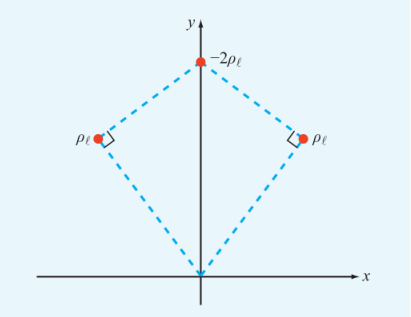
\includegraphics[width=0.6\textwidth]{midterm-1-practice_fig-1.png}
		  \caption{Kite-shaped arrangement of line charges for Problem 4.19.}
		  \label{fig:kite}
		\end{figure}

		Given that we have to infinite lines of charge, we can use the formula derived in the previous question to find the resultant electric field at any point \(P=(r,\phi,0)\) on the \(x-y\) axis, 
		\[
		  \vec{E} = \hat{\alpha}_r \ \frac{\rho_l}{2\pi\varepsilon r}.
		\]
		Using the superposition principle, which allows us to sum the effects of different sources of charge at a given point, and assuming that the distance between the two lines of charges at the sides and the origin is \(r\) and the distance to the central line of charge is \(y\), we may express the total electric field at \(P=(0,0,0)\) as 
		\[
			\vec{E}_{total} = \hat{\alpha}_{r_1}\frac{\rho_l}{2\pi\varepsilon r} + \hat{\alpha}_{r_2}\frac{\rho_l}{2\pi\varepsilon r} - \hat{\alpha}_{-y} \frac{2\rho_l}{2\pi\varepsilon y}.
		\] 
		Assume that the distance between the origin and either of the two lines of charge at the side is \(a\) and the angle between these distances and the \(y\) axis is \(\theta\). Since these two lines are charge are also symmetric on either side of the \(y\) axis, their \(x\) components cancel out, and their total influence is twice their projection onto the \(y\) axis, in the negative \(y\) direction. 

		First, in terms of \(a\) and \(\theta\), the electric field induced at the origin by the central line of charge, all in the \(y\) direction, may be expressed as
		\[
			-\frac{\rho_l \cos{(\theta)}}{\pi \varepsilon a},
		\]
		and the two other lines of charge as
		\[
			\frac{\rho_l \cos{(\theta)}}{\pi \varepsilon a},
		\]
		and so 
		\[
			\frac{\rho_l \cos{(\theta)}}{\pi \varepsilon a}  - \frac{\rho_l \cos{(\theta)}}{\pi \varepsilon a} = 0.
		\]
		\setcounter{subsection}{20}
	\item Three infinite lines of charge, \(\rho_{l_{1}} = 3 \ \mathrm{\frac{nC}{m}}, \ \rho_{l_2} = -3 \ \mathrm{\frac{nC}{m}}\), and \(\rho_{l_3} = 3  \ \mathrm{\frac{nC}{m}}\) are all parallel to the \(z\) axis. If they pass through the respective points \((0,-b)\), \((0,0)\), and \((0,b)\) in the \(x-y\) plane, find the electric field at \((a,0,0).\) Evaluate your result for \(a=2 \ \mathrm{cm}\) and \(b = 1 \ \mathrm{cm}\).
		
		Similar to the previous problem, the two lines of charge at \((0,-b)\) and \((0,b)\) cancel each other's \(y\) components due to symmetry.

		The central line of charge at \((0,0)\) induces an electric field that points solely in the negative \(x\) direction, and may be described at any point \((a,0,0)\)as 
		\[
			\hat{\alpha}_x \frac{-3}{2 \pi \varepsilon a}.
		\]
		Then, the \(x\) components of the other two lines of charge may be described as
		\[
			\hat{\alpha}_x \frac{3a}{2\pi\varepsilon (a^2+b^2)}.
		\]
		Summing the two to find the total electric field at \((a,0,0)\),
		\[
		\vec{E}_a = \hat{\alpha}_x \frac{3}{2\pi\varepsilon} (\frac{a}{(a^2+b^2)}-\frac{1}{a}).
		\]
		\setcounter{subsection}{25}
	\item The electric flux density inside a dielectric sphere of radius \(a\) centered at the origin is given by 
		\[
			\vec{D} = \hat{\alpha_R}\rho_0 R \ \mathrm{\frac{C}{m^2}}
		\]
		where \(\rho_0\) is a constant. Find the total charge inside the sphere.

		Using Gauss's Law,
		\[
		  \oint_{S}\vec{D}\cdot d \vec{s} = Q,
		\]
		and assuming \(d \vec{s} = d \vec{R}\), then \(Q\) is given by
		\[
			Q = \int_{0}^{2\pi} \int_{0}^{\pi} \rho_0 a (a^2 \sin{(\theta})) \ d\phi \ d\theta = \rho_0 4\pi a^3 \ \mathrm{C}.
		\]
		\setcounter{subsection}{29}
	\item A spherical shell with outer radius \(b\) surrounds a charge-free cavity of radius \(a < b\) (Fig. 2). If the shell contains a charge density given by 
		\[
			\rho_v = -\frac{\rho_{v0}}{R^2}, \ \ a \leq R \leq b,
		\]
		where \(\rho_{v0}\) is a positive constant, determine \(\vec{D}\) in all regions.
		
		Again using Gauss's Law, we can derive \(\vec{D}\) from the amount of charge contained within a sphere. Since there is no charge contained within a sphere of radius \(0 < r < a\), there is no electric flux in this region. 

		In the next region, where \(a < r < b\), the charge is dependent on the radius, so, integrating at each point \(r\), 
		\[
			\vec{D} = 4\pi R^2 = Q = 4\pi\int_{a}^{R} \rho_{v0}\ dr,
		\]
		and so, 
		\[
			\vec{D} = \hat{\alpha_r}\frac{\rho_{v0}(R-a)}{R^2} \ \mathrm{\frac{C}{m^2}}
		\]
		in this region.

		Finally, the electric flux outside the sphere is given by 
		\[
			\vec{D} = 4\pi R^2 = Q = 4\pi\rho_{v0}(b-a) \ \mathrm{C},
		\]
		and so flux density in this region is 
		\[
			\vec{D} = \hat{\alpha_r}\frac{\rho_{v0}(b-a)}{R^2} \ \mathrm{\frac{C}{m^2}}
		\]
		\begin{figure}[H]
		  \centering
		  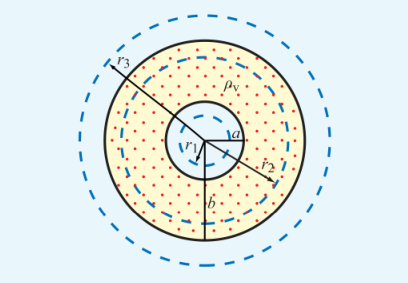
\includegraphics[width=0.6\textwidth]{midterm-1-practice_fig-2.png}
		  \caption{Problem 4.29}
		  \label{fig:shell}
		\end{figure}
		\setcounter{subsection}{30}
	\item A square in the \(x-y\) plane in free space has a point charge of \(+Q\) at corner \(\frac{a}{2}, \frac{a}{2}\), the same at corner \(\frac{a}{2}, \frac{-a}{2}\), and a point charge of \(-Q\) at each of the other two corners.
		\begin{enumerate}[label=(\alph*)]
			\item Find the electric potental at any point \(P\) along the \(x\) axis. 

				For this problem, we'll first sum the influence of the point charges at any point along the \(x\) axis, where the symmetry of the two corresponding charges cancels their \(y\) components,
				\[
				  \vec{E} = \hat{\alpha}_x\frac{Q}{2\pi\varepsilon_0}(\frac{1}{\sqrt{x^2-ax+\frac{a^2}{2}}} - \frac{1}{\sqrt{x^2 + ax + \frac{a^2}{2}}}).
				\]
				However, we may also derive the expression for electric potential due to multiple point charges as 
				\[
				  V = \frac{q}{4\pi\varepsilon |\vec{r} - \vec{r}_1|}.
				\]
				Summing the influence of each point,
				\[
					V = \frac{1}{4\pi\varepsilon_0} \sum_{N}^{i=1}\frac{q_i}{|\vec{r} - \vec{r}_1|}.
				\]
				For the positive \(Q\)s, \(|\vec{r}-\vec{r}_1| = \sqrt{x^2 - ax + \frac{a^2}{4}}\), and for the negative \(Q\)s, \(|\vec{r}-\vec{r}_1| = \sqrt{x^2 + ax + \frac{a^2}{4}}\), so
				\[
				V = \frac{1}{2\pi\varepsilon_0} (\frac{Q}{\sqrt{x^2 - ax + \frac{a^2}{2}}} - \frac{Q}{\sqrt{x^2 + ax + \frac{a^2}{2}}}).
				\]
			\item Evaluate \(V\) at \(x=\frac{a}{2}\).

				Using the formula above, 
				\[
				  V = \frac{2Q}{2\pi\varepsilon_0 a}(1 - \frac{1}{\sqrt{5}}).
				\]
		\end{enumerate}
	\setcounter{subsection}{48}
	\item With reference to Fig. 3, find \(\vec{E}_1\) if 
		\[
			\vec{E}_2 = \hat{\alpha}_x3 - \hat{\alpha}_y + \hat{\alpha}_z2 \ \mathrm{\frac{V}{m}},
		\]
		\(\varepsilon_1 = 2\varepsilon_0, \ \varepsilon_2 = 18\varepsilon_0\), and the boundary has a surface charge density \(\rho_s = 3.54 \times 10^{-11} \ \mathrm{\frac{C}{m^2}}.\) What angle does \(\vec{E}_2\) make with the \(z\) axis?

		Firstly, tangential components of \(\vec{E}\) at a boundary are continuous, and so
		\[
			\vec{E}_{1t} = \hat{\alpha}_x3 - \hat{\alpha}_y \ \mathrm{\frac{V}{m}}.
		\]
		
		To find the normal component of \(\vec{E}_1\), we'll use the electric flux density and permittivity of each material. Since \(\vec{D} = \varepsilon \vec{E}\), 
		\[
		  \vec{D}_2 = \varepsilon_0(\hat{\alpha}_x54 - \hat{\alpha}_y18 + \hat{\alpha_z}36).
		\]
		Taking the components normal to the \(x-y\)	plane,
		\[
			\vec{D}_{2n} = \varepsilon_0(\hat{\alpha}_z36),
		\]
		and so dividing by \(\varepsilon_2 = \varepsilon_02\),
		\[
			\vec{D}_{1n} = \rho_s + \vec{D}_{2n} = \hat{\alpha}_z(3.54 \times 10^{-11} + 36) \approx \hat{\alpha}_z36
		\]
		and 
		\[
			\vec{E}_1 = \hat{\alpha}_x3-\hat{\alpha}_y + \hat{\alpha}_z18 \ \mathrm{\frac{V}{m}}.
		\]

		Then, finding the angle of \(\vec{E}_2\) with the \(z\) axis using the dot product, 
		\[
		\cos^{-1}{(\frac{18}{18.28})} \approx 10\degree.
		\]
		\begin{figure}[H]
		  \centering
		  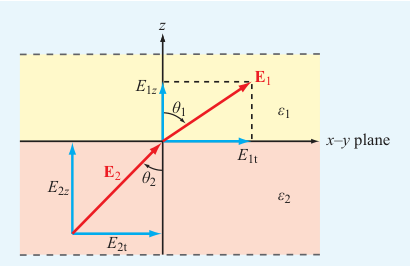
\includegraphics[width=0.6\textwidth]{midterm-1-practice_fig-3.png}
		  \caption{Application of boundary conditions at the interface between two dielectric media.}
		  \label{fig:boundary}
		\end{figure}
		\setcounter{subsection}{51}
	\item Fig. 4 shows three planar dielectric slabs of equal thickness but with different dielectric constants. If \(\vec{E}_0\) in air makes an angle of \(45\degree\) with respect to the \(z\) axis, find the angle of \(\vec{E}\) in each of the other layers.
		\begin{figure}[H]
		  \centering
		  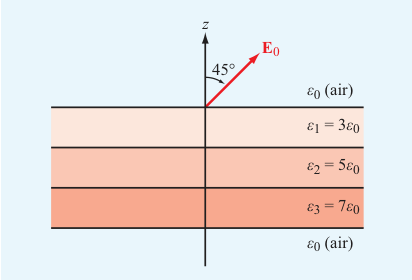
\includegraphics[width=0.6\textwidth]{midterm-1-practice_fig-4.png}
		  \caption{Dielectric slabs in Problem 4.51.}
		  \label{fig:slabs}
		\end{figure}
		\setcounter{subsection}{58}
	\item The capacitor shown in Fig. 5 consists of two parallel dielectric layers. Use energy considerations to show that the equivalent capacitance of the overall capacitor, \(C\), is equal to the series combination of the capacitances of the individual layers, \(C_1\) and \(C_2\), namely
		\[
		  C = \frac{C_1C_2}{C_1 + C_2},
		\]
		where 
		\begin{align*}
			&C_1 = \varepsilon_1 \frac{A}{d_1} &C_2 = \varepsilon_2 \frac{A}{d_2}.
		\end{align*}
		\begin{figure}[H]
		  \centering
		  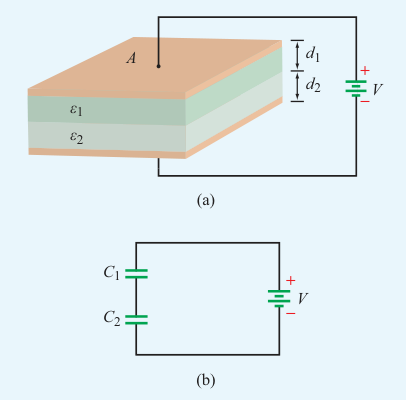
\includegraphics[width=0.6\textwidth]{midterm-1-practice_fig-5.png}
		  \caption{(a) Capacitor with parallel dielectric layers and (b) equivalent circuit.}
		  \label{fig:capacitor}
		\end{figure}
		\setcounter{subsection}{61}
	\item With reference to Fig. 6, charge \(Q\) is located at a distance \(d\) above a grounded half-plane located in the \(x-y\) plane and at a distance \(d\) from another grounded half-plane in the \(x-y\) plane. Use the image method to 
		\begin{enumerate}[label=(\alph*)]
			\item Establish the magnitudes, polarities, and locations of the images of charge \(Q\) with respect to each of the two ground planes (as if each is infinite in extent).
			\item Find the electric potential and electric field at an arbitrary point \(P = (0,y,z).\)
		\end{enumerate}
		\begin{figure}[H]
		  \centering
		  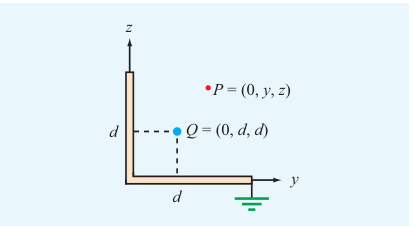
\includegraphics[width=0.6\textwidth]{midterm-1-practice_fig-6.png}
		  \caption{Charge \(Q\) next to two perpendicular, grounded, conducting half-planes.}
		  \label{fig:halfplanes}
		\end{figure}
		\setcounter{subsection}{63}
	\item Use the image method to find the capacitance per unit length of an infinitely long conducting cylinder of radius \(a\) situated at a distance \(d\) from a parallel conducting plane, as shown in Fig. 7.
		\begin{figure}[H]
		  \centering
		  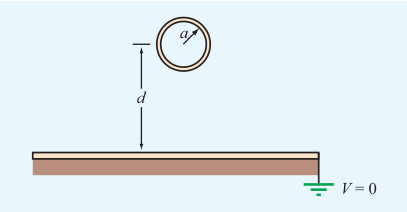
\includegraphics[width=0.6\textwidth]{midterm-1-practice_fig-7.png}
		  \caption{Conducting cylinder above a conducting plane.}
		  \label{fig:cylinder}
		\end{figure}
\end{enumerate}
\end{document}
